\begin{figure*}[thp]
	\center
	\begin{subfigure}{0.85\textwidth}
	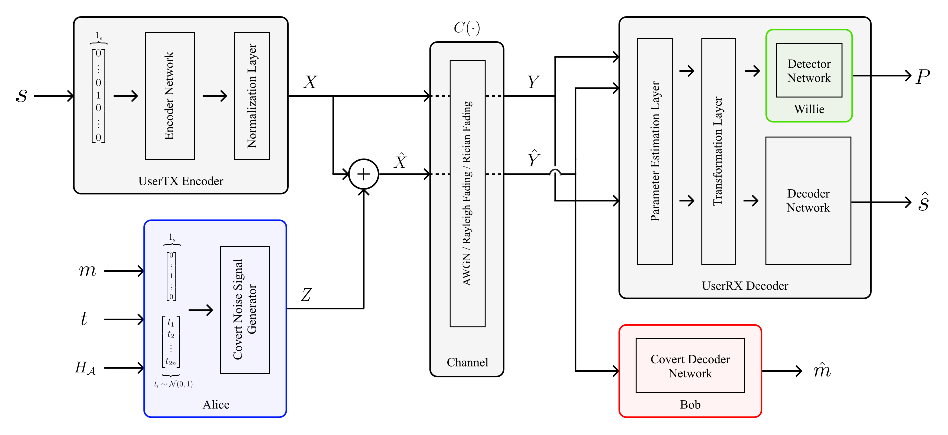
\includegraphics[width=\linewidth]{figs/system_architecture}
	\end{subfigure}
	\caption{Our covert communication scheme over AWGN and Rayelgh fading channels on top of a normal autoencoder-based wireless communication system.}	
	\label{fig:system_architecture}
\end{figure*}
\section{Background On Autoencoder Wireless Systems}
\label{s:background}
An autoencoder-based wireless communication system is an end-to-end learning paradigm that abstracts out the coding and modulation components of a  traditional modular communication system by replacing the transmitter and receiver with DNNs. The encoder (transmitter) first uses a mapping to transform \(k\) bits of data into a message \(s\) where \(s \in \{1,...,M\}\) and \(M = 2^k\). Then it takes this transformed message as an input and generates a signal \(x = E(s) \in \mathbb{R}^{2n}\), which is a real valued vector. This \(2 \times n\) dimensional real valued vector can be treated as an \(n\) dimensional complex vector where \(n\) is the number of channel uses the signal needs to be transmitted over. Then, the channel's noise effect \(z\), which is usually considered to be AWGN, is added to the signal vector. Thus, the received signal at the receiver has noise of the channel added and can be expressed as \(y = x + z\). In case there are many objects in the environment, Rayleigh fading is a more reasonable model for the channel. In this channel model, received signal is given by \(y = h \cdot x + z\), where \(h \sim \mathcal{CN}(0, 1)\) is the fading channel gain. The decoder (receiver) applies the transformation \(D: \mathbb{R}^{2n} \rightarrow M \) to outputs the reconstructed version of the message \(s\), which is denoted as \(\hat{s} = D(y)\).
